\documentclass[11pt,a4paper,reqno]{amsart}

\usepackage[utf8]{inputenc}
\usepackage[T1]{fontenc}
\usepackage{amsmath,amssymb,amsfonts,amsthm,mathtools}
\usepackage{mathrsfs}
\usepackage{microtype}
\usepackage{booktabs}
\usepackage{tabularx}
\usepackage{array}
\usepackage[dvipsnames]{xcolor}
\usepackage{hyperref}
\usepackage{geometry}
\usepackage{enumitem}
\usepackage{graphicx}

\geometry{
  top=2.8cm,
  bottom=2.8cm,
  left=2.6cm,
  right=2.6cm,
  headheight=14pt
}

\definecolor{navyblue}{RGB}{16, 44, 87}
\definecolor{darkforest}{RGB}{20, 80, 45}
\definecolor{burgundy}{RGB}{128, 20, 36}

\hypersetup{
  colorlinks=true,
  linkcolor=navyblue,
  citecolor=darkforest,
  urlcolor=burgundy,
  pdfauthor={Reinaldo Maia Silva-Filho},
  pdftitle={Simplicial Quantum Gravity on Delta4 x Delta2: A Two-Scale Spectral Dimension, L-infinity Minimax Foliations, and Conjectures on Gauge and Flavor Structure}
}

% --- Theorem Environments ---
\newtheorem{theorem}{Theorem}[section]
\newtheorem{lemma}[theorem]{Lemma}
\newtheorem{proposition}[theorem]{Proposition}
\newtheorem{corollary}[theorem]{Corollary}

\theoremstyle{definition}
\newtheorem{definition}[theorem]{Definition}
\newtheorem{example}[theorem]{Example}
\newtheorem{remark}[theorem]{Remark}
\newtheorem{hypothesis}[theorem]{Hypothesis}
\newtheorem{conjecture}[theorem]{Conjecture}

\numberwithin{equation}{section}

% --- Custom Notations ---
\newcommand{\R}{\mathbb{R}}
\newcommand{\C}{\mathbb{C}}
\newcommand{\N}{\mathbb{N}}
\newcommand{\Z}{\mathbb{Z}}
\newcommand{\Sph}{\mathbb{S}}
\newcommand{\Hyp}{\mathbb{H}}
\newcommand{\Id}{\mathrm{Id}}
\newcommand{\Tr}{\operatorname{Tr}}
\newcommand{\rank}{\operatorname{rank}}
\newcommand{\supp}{\operatorname{supp}}
\newcommand{\Lip}{\operatorname{Lip}}
\newcommand{\BV}{\operatorname{BV}}
\newcommand{\Area}{\operatorname{Area}}
\newcommand{\Vol}{\operatorname{Vol}}
\newcommand{\Ric}{\operatorname{Ric}}
\newcommand{\Hess}{\operatorname{Hess}}
\newcommand{\reach}{\operatorname{reach}}
\newcommand{\II}{\mathrm{I\!I}}
\newcommand{\cutnorm}[1]{\|#1\|_{\square}}
\newcommand{\norm}[1]{\left\|#1\right\|}
\newcommand{\inner}[2]{\left\langle #1, #2 \right\rangle}
\newcommand{\dif}{\,\mathrm{d}}
\newcommand{\abs}[1]{\left|#1\right|}
\newcommand{\SU}{\mathrm{SU}}
\newcommand{\SO}{\mathrm{SO}}
\newcommand{\U}{\mathrm{U}}
\newcommand{\Pl}{\mathrm{Planck}}

\title[Simplicial Quantum Gravity on $\Delta_4 \times \Delta_2$]{Simplicial Quantum Gravity on $\Delta_4 \times \Delta_2$:\\ A Two-Scale Spectral Dimension, $L^\infty$-Minimax Foliations,\\ and Conjectures on Gauge and Flavor Structure}

\author{Reinaldo Maia Silva-Filho}
\address{Programa de P\'os-Gradua\c{c}\~ao em Estat\'istica e Experimenta\c{c}\~ao Agropecu\'aria (PPGEE/DES)\\
Departamento de Estat\'istica (DES), Universidade Federal de Lavras (UFLA)\\
Caixa Postal 3037, CEP 37200-900, Lavras, Minas Gerais, Brazil}
\email{reinaldo.filho1@estudante.ufla.br}

\thanks{This research was supported by the Coordena\c{c}\~ao de Aperfei\c{c}oamento de Pessoal de N\'ivel Superior (CAPES) -- Finance Code 001. Code repository (Lean~4 naming skeleton and numerical scripts): \url{https://github.com/reinaldomsilvafilho-netizen/quantum-gravity-lean4}.}

\date{\today}

\begin{document}

\begin{abstract}
We study a mathematical framework for quantum geometry and gauge fields formulated on the simplicial product $\mathcal{M} = \Delta_4 \times \Delta_2$, where $\Delta_4$ is the standard 4-simplex used as a model of a spacetime cell and $\Delta_2$ is an internal flavor 2-simplex. The framework combines an $L^\infty$-minimax extrinsic curvature principle with non-local integro-differential operators on simplices. We separate proved statements, phenomenological models and conjectures throughout.

The proved results are elementary but exact:
(1) for the \emph{assumed} isotropic two-scale diffusion symbol $k^2 + \ell_P^2 k^4$ in four Euclidean dimensions we give a closed form for the spectral dimension $d_s(\tau)$, which interpolates between $d_s = 4$ at large diffusion times and $d_s = 2$ at short ones, the same end values as in Causal Dynamical Triangulations and in Ho\v{r}ava--Lifshitz gravity (where they arise from a different, anisotropic operator); the symbol is not derived from the simplicial operators, and in Lorentzian signature its isotropic $k^4$ term carries a ghost;
(2) on a spacelike hypersurface whose second fundamental form is bounded in operator norm by $\kappa^*$, one has $\sigma_{ij}\sigma^{ij} \le 3(\kappa^*)^2 - \frac{1}{3}K^2$, and the vacuum Hamiltonian constraint confines the scalar curvature to the sharp interval $2\Lambda - 6(\kappa^*)^2 \le {}^{(3)}R \le 2\Lambda + 2(\kappa^*)^2$; in FLRW the same cutoff bounds the Hubble rate and hence the energy density, but it does not by itself produce a bounce;
(3) in an obstacle-problem model of wave-packet localization, Caffarelli's optimal $C^{1,1}$ regularity applies under its standard hypotheses.
We also record what the framework does \emph{not} give: phase-space volumes on $\mathbb{C}P^{N-1}$ of the natural attraction regions are state-independent and do not reproduce the Born rule; the Dirac--K\"ahler formulation yields four degenerate tastes rather than an evasion of the Nielsen--Ninomiya theorem, and three generations enter as an input through the choice of $\Delta_2$; the Koide relation $Q_l = 2/3$ admits an $S_3$ reformulation but is not derived; and the alternating sum of facet volumes of $\Delta_4$ does not vanish, so the chain identity $\partial \circ \partial = 0$ gives no cancellation of vacuum energy. A Yang--Mills mass gap on the Gribov region and the condensation of graphon Ricci flows into smooth four-dimensional geometries are stated as conjectures, with the missing steps identified.

Order-of-magnitude estimates show that Planck-suppressed observational signatures of the kind considered here lie many orders of magnitude below current and planned experimental reach. The accompanying Lean~4 files are a naming skeleton and do not verify the mathematics of this paper.
\end{abstract}

\maketitle

\tableofcontents

% =========================================================================
\section{Introduction and the \texorpdfstring{$\Delta_4 \times \Delta_2$}{Delta4 x Delta2} Variational Principle}
\label{sec:intro}
% =========================================================================

The unification of General Relativity (GR) and the Standard Model (SM) of particle physics within a single non-perturbative framework remains the preeminent problem of fundamental theoretical physics \cite{jaffe2006quantum, ambjorn2012nonperturbative}. When smooth pseudo-Riemannian manifolds $(M^4, g)$ and the Einstein--Hilbert action are extrapolated to trans-Planckian scales ($\ell \ll \ell_P = \sqrt{\hbar G/c^3} \approx 1.616 \times 10^{-35}\text{ m}$), one meets ultraviolet divergences and perturbative non-renormalizability \cite{goroff1986ultraviolet} and curvature singularities (Big Bang and black holes) \cite{hawking1970singularities}.

This paper does not resolve these problems. Its aim is narrower: to formulate a candidate framework, which we call \emph{Simplicial Quantum Gravity (SQG)}, and to record precisely which of its statements are proved, which are models resting on stated assumptions, and which remain conjectural. Statements labelled \emph{Theorem} or \emph{Proposition} are proved here or in the cited literature; statements labelled \emph{Conjecture} are not; \emph{Remarks} record heuristics, models, and negative results. The framework is formulated on the Cartesian product
\begin{equation}
    \label{eq:base_manifold}
    \mathcal{M} = \Delta_4 \times \Delta_2,
\end{equation}
where $\Delta_4$ is the regular 4-simplex (the pentachoron, used as a model of a spacetime cell) and $\Delta_2$ is the internal 2-simplex (the flavor triangle, whose three vertices label fermion families). In place of $C^\infty$ smoothness and $L^2$ kinetic integrals we \emph{postulate} an $L^\infty$-minimax bound, coupled to non-local operators on the simplex:
\begin{equation}
    \label{eq:minimax_functional_master}
    \mathcal{S}_\infty[g, A, \Psi] = \operatorname{ess\,sup}_{x \in \mathcal{M}} \left\{ \|\II_g(x)\|_{\mathrm{op}} + \lambda_A \|F_A(x)\|_{\mathrm{op}} + \lambda_\Psi \|\mathcal{D}_{\mathrm{DK}} \Psi(x)\|_{\mathrm{op}} \right\} \le \ell_P^{-1},
\end{equation}
where the couplings $\lambda_A$ (dimension of length) and $\lambda_\Psi$ make the three terms dimensionally commensurate. The bound \eqref{eq:minimax_functional_master} is an assumption of the framework; no dynamics that enforces it is derived here.

\subsection{Geometric Structure of the Spacetime 4-Simplex \texorpdfstring{$\Delta_4$}{Delta4}}
The standard 4-simplex $\Delta_4$ is defined in barycentric coordinates by:
\begin{equation}
    \label{eq:delta4_def}
    \Delta_4 \coloneqq \left\{ \mathbf{x} = (x_0, x_1, x_2, x_3, x_4) \in \R_{\ge 0}^5 \;\middle|\; \sum_{i=0}^4 x_i = 1 \right\}.
\end{equation}
We equip the interior of $\Delta_4$ with the Fisher--Rao metric of the categorical distributions $\mathbf{x}$, which is also the quantum Fisher metric of the commuting family of diagonal density matrices $\rho_{\mathbf{x}} = \operatorname{diag}(x_0, \dots, x_4)$:
\begin{equation}
    \label{eq:qfi_metric}
    g_{\mu\nu}(\mathbf{x}) = \sum_{i=0}^4 \frac{1}{x_i} \frac{\partial x_i}{\partial x^\mu} \frac{\partial x_i}{\partial x^\nu}, \qquad D_{\mathrm{KL}}(\rho_{\mathbf{x}} \,\|\, \rho_{\mathbf{x} + \dif \mathbf{x}}) = \frac{1}{2}\, g_{\mu\nu}\, \dif x^\mu \dif x^\nu + \mathcal{O}(|\dif\mathbf{x}|^3),
\end{equation}
where $x^\mu$ ($\mu = 1, \dots, 4$) are coordinates on $\Delta_4$ and lengths are measured in units of $\ell_P$. This metric is Riemannian; relating it to a Lorentzian spacetime metric is not attempted here.
The topological boundary $\partial \Delta_4$ consists of five tetrahedral 3-cells $\sigma_3^{(i)}$ ($i = 0, \dots, 4$), the facets opposite the vertices. As simplicial chains,
\begin{equation}
    \label{eq:boundary_homology}
    \partial \Delta_4 = \sum_{i=0}^4 (-1)^i \sigma_3^{(i)}, \qquad \partial(\partial \Delta_4) = 0,
\end{equation}
so the boundary is a closed 3-cycle. By Stokes' theorem the flux of an exact 3-form through $\partial\Delta_4$ vanishes. The identity concerns chains and exact forms; it does not make the alternating sum of facet \emph{volumes} vanish (Remark~\ref{rem:vacuum_cancellation}).

\subsection{Geometric Structure of the Flavor 2-Simplex \texorpdfstring{$\Delta_2$}{Delta2}}
The internal flavor space is the standard 2-simplex:
\begin{equation}
    \label{eq:delta2_def}
    \Delta_2 \coloneqq \left\{ \mathbf{y} = (y_1, y_2, y_3) \in \R_{\ge 0}^3 \;\middle|\; y_1 + y_2 + y_3 = 1 \right\}.
\end{equation}
The automorphism group of $\Delta_2$ is the symmetric group $S_3 \cong D_3$ of order 6. It permutes the three vertices, and the corresponding permutation representation on $\mathcal{H}_{\mathrm{flavor}} = \R^3$ (or $\C^3$) decomposes into irreducible representations as
\begin{equation}
    \label{eq:s3_decomposition}
    \mathcal{H}_{\mathrm{flavor}} \cong \mathbf{1}_{\mathrm{trivial}} \oplus \mathbf{2}_{\mathrm{standard}}.
\end{equation}
The number of vertices, $N_g = \dim(\Delta_2) + 1 = 3$, equals the number of observed chiral generations. This is an input of the model: choosing the flavor space to be a 2-simplex is equivalent to choosing three generations, so the equality is not a prediction.

% =========================================================================
\section{Dirac--K\"ahler Differential Forms and Lattice Fermion Doubling}
\label{sec:dirac_kahler}
% =========================================================================

A long-standing obstacle in discrete quantum field theory is the Nielsen--Ninomiya no-go theorem \cite{nielsen1981absence}: a local, hermitian, translation-invariant lattice fermion action with the continuum chiral symmetry necessarily has species doubling (the naive discretization in $d = 4$ has $2^d = 16$ species).

In the SQG framework, fermions are not formulated as pointlike spinor fields $\psi_\alpha(x)$, but as \emph{inhomogeneous Dirac--K\"ahler differential forms} $\Psi \in \Omega^*(\Delta_4)$ \cite{kahler1962innere, becher1982dirac, rabin1982homology}:
\begin{equation}
    \label{eq:dirac_kahler_field}
    \Psi = \sum_{p=0}^4 \psi_{(p)}, \quad \psi_{(p)} = \frac{1}{p!} \psi_{\mu_1 \dots \mu_p} \dif x^{\mu_1} \wedge \dots \wedge \dif x^{\mu_p}.
\end{equation}
The classical Dirac operator $\gamma^\mu D_\mu$ is replaced by the Hodge--de~Rham operator:
\begin{equation}
    \label{eq:hodge_de_rham}
    \mathcal{D}_{\mathrm{DK}} \coloneqq \dif - \delta = \dif - \star \dif \star,
\end{equation}
where $\dif$ is the exterior derivative, $\delta$ is the codifferential, and $\star$ is the Hodge star operator on $\Delta_4$.

\begin{proposition}[Clifford Structure of Dirac--K\"ahler Fields]
\label{thm:nielsen_ninomiya_evasion}
Let $\Psi \in \Omega^*(\Delta_4)$ be an inhomogeneous Dirac--K\"ahler field with the action
\begin{equation}
    \mathcal{S}_{\mathrm{fermion}} = \int_{\Delta_4} \langle \Psi, (\dif - \delta) \Psi \rangle \dif \mu_{\Delta_4}.
\end{equation}
Then:
\begin{enumerate}[label=(\roman*)]
    \item The Clifford product of forms, defined on 1-forms by
    \begin{equation}
        v \vee w = v \wedge w + g^{-1}(v, w), \quad \forall v, w \in \Omega^1(\Delta_4),
    \end{equation}
    and extended by $v \vee \omega = v \wedge \omega + \iota_{v^\sharp}\, \omega$, makes $\Omega^*_x(\Delta_4)$ at each point a Clifford algebra of the metric $g$; for the Riemannian metric \eqref{eq:qfi_metric} this is $\mathcal{C}\ell(4)$, and $\mathcal{C}\ell(1,3)$ requires a Lorentzian metric.
    \item The $16$-dimensional exterior algebra decomposes into four minimal left ideals, each carrying a $4$-component Dirac spinor \cite{kahler1962innere, becher1982dirac}.
\end{enumerate}
\end{proposition}
\begin{proof}
The exterior algebra has dimension $\sum_{p=0}^4 \binom{4}{p} = 16 = 2^4$, and $\mathcal{C}\ell(4) \cong M_4(\C)$ after complexification. A complexified matrix algebra $M_4(\C)$ is the direct sum of four minimal left ideals (its columns), each isomorphic to $\C^4$ \cite{kahler1962innere, becher1982dirac, rabin1982homology}.
\end{proof}

\begin{remark}[Doubling and the number of generations]
\label{rem:nn_caveats}
The four spinors of Proposition~\ref{thm:nielsen_ninomiya_evasion}(ii) are four degenerate \emph{tastes}: this is the content of the Becher--Joos lattice construction \cite{becher1982dirac}, which is equivalent to staggered fermions. On a lattice the Dirac--K\"ahler field therefore does not evade the Nielsen--Ninomiya theorem; it reorganizes the $16$ naive doublers into four tastes of $4$-component spinors \cite{becher1982dirac, rabin1982homology}. Non-locality can violate a hypothesis of the theorem, but the operator of Definition~\ref{def:beta_laplacian} has an integrable kernel (Remark~\ref{rem:kernel_integrable}), and we have not shown that a fermion action built from it has no spurious zeros, is free of the known pathologies of non-local lattice derivatives, or has the correct continuum limit. Whether doubling is absent in this framework is therefore open. Finally, four tastes do not match three generations, and $N_g = \dim(\Delta_2) + 1 = 3$ is an input (Section~\ref{sec:intro}), not a consequence of the representation theory of $S_3$.
\end{remark}

% =========================================================================
\section{The Fractional Simplicial Beta-Laplacian and Spectral Dimension Flow}
\label{sec:beta_laplacian}
% =========================================================================

As a candidate non-local operator on the simplex we consider the \emph{Simplicial Beta-Laplacian} $(-\Delta_{\Delta_m})^\alpha$.

\begin{definition}[Simplicial Beta-Laplacian]
\label{def:beta_laplacian}
Let $\Delta_m$ be the standard $m$-simplex equipped with the Dirichlet probability measure $\dif \mu_{\mathbf{a}}(\mathbf{x}) = \frac{1}{\mathrm{B}(\mathbf{a})} \prod_{i=1}^{m+1} x_i^{a_i - 1} \dif \mathbf{x}$. The fractional operator of order $\alpha \in (0, 1)$ on the Sobolev space $H^\alpha(\Delta_m, \mu_{\mathbf{a}})$ is defined by:
\begin{equation}
    \label{eq:beta_laplacian_formula}
    (-\Delta_{\Delta_m})^\alpha u(\mathbf{x}) \coloneqq \operatorname{P.V.} \int_{\Delta_m} \frac{u(\mathbf{x}) - u(\mathbf{y})}{\mathcal{K}_\alpha(\mathbf{x}, \mathbf{y})} \dif \mu_{\mathbf{a}}(\mathbf{y}) + B_\alpha(\mathbf{x}) u(\mathbf{x}),
\end{equation}
where the convolution kernel is:
\begin{equation}
    \mathcal{K}_\alpha(\mathbf{x}, \mathbf{y}) \coloneqq C(m, \alpha) \prod_{i=1}^m |x_i - y_i|^{1 - \alpha},
\end{equation}
and the boundary barrier potential is:
\begin{equation}
    \label{eq:boundary_barrier}
    B_\alpha(\mathbf{x}) \coloneqq \int_{\partial \Delta_m} \frac{\dif \sigma(\mathbf{y})}{\|\mathbf{x} - \mathbf{y}\|^{m + 2\alpha - 1}}.
\end{equation}
\end{definition}

The boundary potential $B_\alpha(\mathbf{x})$ diverges as $\mathbf{x} \to \partial \Delta_m$. As a non-negative potential term it acts as a killing rate: the associated semigroup is sub-Markovian and does not conserve probability. Whether it confines the process to the simplex in a stronger sense has not been analysed.

\begin{remark}[The kernel is integrable]
\label{rem:kernel_integrable}
The weight $1/\mathcal{K}_\alpha(\mathbf{x}, \mathbf{y}) = C(m,\alpha)^{-1} \prod_i |x_i - y_i|^{\alpha - 1}$ in \eqref{eq:beta_laplacian_formula} is locally integrable for $\alpha > 0$, so no principal value is needed. The first term of \eqref{eq:beta_laplacian_formula} is therefore not a fractional Laplacian of order $2\alpha$ (whose kernel behaves like $\|\mathbf{x} - \mathbf{y}\|^{-m - 2\alpha}$), and it does not have the symbol $|k|^{2\alpha}$. The same holds for the Beta-kernel operators of \cite{silvafilho2026treatise} (Chapters~3--4), whose symbols are bounded. The spectral-dimension results below concern model symbols and do not follow from Definition~\ref{def:beta_laplacian}.
\end{remark}

For $\alpha > 0$ let $(-\Delta)^\alpha$ denote the Fourier multiplier with symbol $|k|^{2\alpha}$ on $\R^m$. Its heat kernel has diagonal $P(\tau) = C(m,\alpha)\,\tau^{-m/(2\alpha)}$, so the spectral dimension $d_s \coloneqq -2\, \dif \ln P / \dif \ln \tau = m/\alpha$ is \emph{constant} \cite{silvafilho2026treatise}. A running spectral dimension therefore needs a symbol with two scales. Numerical simulations of Causal Dynamical Triangulations (CDT) in $3+1$ dimensions show $d_s$ decreasing from $\approx 4$ at large diffusion times to $\approx 2$ at short ones \cite{ambjorn2005spectral}, and similar short-distance values occur in several other approaches \cite{carlip2017dimension}. In Ho\v{r}ava--Lifshitz gravity with anisotropic scaling exponent $z$ in $3+1$ dimensions the ultraviolet value is $d_s = 1 + 3/z$, so $d_s = 2$ requires $z = 3$, while $z = 2$ (a spatial $k^4$ term) gives $5/2$ \cite{horava2009spectral}. In $2+1$ dimensions, Sotiriou, Visser and Weinfurtner showed that Ho\v{r}ava--Lifshitz-type dispersion relations reproduce the CDT flow of $d_s$ to high accuracy \cite{sotiriou2011spectral}. Here we consider a different, isotropic operator.

\begin{proposition}[Closed Form of the Spectral Dimension for a Two-Scale Symbol]
\label{thm:spectral_dimension_flow}
Consider the heat equation on $\R^4$ with the \emph{assumed} isotropic Euclidean symbol $k^2(1 + \ell_P^2 k^2)$, and let $P(\tau) = P(\tau; \mathbf{x}, \mathbf{x})$ be the diagonal of its heat kernel. With $z \coloneqq \sqrt{\tau}/(2\ell_P)$,
\begin{equation}
    \label{eq:ds_return_probability}
    P(\tau) = \frac{1}{(2\pi)^4} \int_{\R^4} e^{-\tau (k^2 + \ell_P^2 k^4)} \dif^4 k = \frac{1}{32 \pi^2 \ell_P^2 \tau} \left[ 1 - \sqrt{\pi}\, z\, e^{z^2} \operatorname{erfc}(z) \right],
\end{equation}
and the spectral dimension $d_s(\tau) \coloneqq -2\, \dif \ln P / \dif \ln \tau$ is
\begin{equation}
    \label{eq:ds_analytic_formula}
    d_s(\tau) = 1 - \frac{\tau}{2\ell_P^2} + \left[ 1 - \frac{\sqrt{\pi \tau}}{2\ell_P} \exp\!\left(\frac{\tau}{4\ell_P^2}\right) \operatorname{erfc}\!\left(\frac{\sqrt{\tau}}{2\ell_P}\right) \right]^{-1}.
\end{equation}
Consequently $\lim_{\tau \to 0} d_s(\tau) = 2$ and $\lim_{\tau \to \infty} d_s(\tau) = 4$, with $d_s = 4 - 12\ell_P^2/\tau + \mathcal{O}(\ell_P^4/\tau^2)$ as $\tau \to \infty$.
\end{proposition}
\begin{proof}
In polar coordinates, with $u = k^2$, $P(\tau) = \frac{1}{16\pi^2} \int_0^\infty u\, e^{-\tau u - \tau \ell_P^2 u^2} \dif u$. Completing the square, $\tau u + \tau \ell_P^2 u^2 = \tau\ell_P^2 (u + \frac{1}{2\ell_P^2})^2 - z^2$, and the two elementary Gaussian integrals give \eqref{eq:ds_return_probability}. Taking the logarithmic derivative yields \eqref{eq:ds_analytic_formula}. As $z \to 0$, $\operatorname{erfc}(z) = 1 - 2z/\sqrt{\pi} + \mathcal{O}(z^3)$ gives $d_s \to 1 + 1 = 2$. As $z \to \infty$, $\sqrt{\pi}\, z\, e^{z^2} \operatorname{erfc}(z) = 1 - 1/(2z^2) + 3/(4z^4) + \mathcal{O}(z^{-6})$, so the reciprocal bracket is $2z^2 + 3 + \mathcal{O}(z^{-2})$; it cancels the term $-\tau/(2\ell_P^2) = -2z^2$ and gives $d_s \to 4$. We have checked \eqref{eq:ds_return_probability} and \eqref{eq:ds_analytic_formula} against direct numerical quadrature for $\tau/\ell_P^2 \in [10^{-3}, 10^2]$ (script \texttt{check\_\allowbreak sqg\_\allowbreak formulas.py} in the accompanying repository).
\end{proof}

\begin{remark}[Scope of the diffusion model]
\label{rem:ds_scope}
The formula \eqref{eq:ds_analytic_formula} gives the spectral dimension of this particular diffusion model. The symbol is an assumption: it is not induced by the kernel of Definition~\ref{def:beta_laplacian} (Remark~\ref{rem:kernel_integrable}), and whether quantum spacetime diffuses according to it is not established. The operator is isotropic in four Euclidean dimensions, so its $k^4$ term contains fourth time derivatives. Continued to Lorentzian signature, the propagator $1/[p^2(1 + \ell_P^2 p^2)]$ has, besides the massless pole, a pole at $p^2 = -1/\ell_P^2$ with negative residue, i.e.\ a ghost. Ho\v{r}ava--Lifshitz gravity avoids higher time derivatives by using an \emph{anisotropic} operator, for which the ultraviolet value is $d_s = 1 + 3/z$ \cite{horava2009spectral}; the anisotropic operator $\omega^2 + k^2 + \ell_P^2 k^4$ ($z = 2$) gives $5/2$, not $2$. That $d_s = 2$ at short scales is associated with power-counting renormalizability of gravity is a heuristic argument used in Ho\v{r}ava--Lifshitz gravity; it is not established here.
\end{remark}

% =========================================================================
\section{\texorpdfstring{$L^\infty$}{L-infinity}-Minimax Foliations and ADM Hamiltonian Regularization}
\label{sec:minimax_adm}
% =========================================================================

In the canonical Arnowitt--Deser--Misner (ADM) $3+1$ formulation of General Relativity \cite{arnowitt1962dynamics, dirac1964lectures, dewitt1967quantum}, spacetime is foliated by spacelike hypersurfaces $\Sigma_t$ with metric $\dif s^2 = -N^2 \dif t^2 + \gamma_{ij}(\dif x^i + N^i \dif t)(\dif x^j + N^j \dif t)$, where $N$ is the lapse function and $N^i$ is the shift vector.

The classical constraint equations on $\Sigma_t$ (units $c = 1$, cosmological constant $\Lambda$, energy density $\rho$ and momentum density $J_i$ measured by the normal observer) consist of the Hamiltonian constraint $\mathcal{H} = 0$ and the momentum constraints $\mathcal{H}_i = 0$:
\begin{align}
    \label{eq:wdw_constraint}
    \mathcal{H} &= {}^{(3)}R - 2\Lambda + \frac{2}{3}K^2 - \sigma_{ij}\sigma^{ij} - 16\pi G_N \rho = 0, \\
    \label{eq:momentum_constraint}
    \mathcal{H}_i &= D_j \left( K^j{}_i - \delta^j{}_i K \right) - 8\pi G_N J_i = 0,
\end{align}
where $K = \gamma^{ij} K_{ij}$ is the mean extrinsic curvature and $\sigma_{ij} = K_{ij} - \frac{1}{3} K \gamma_{ij}$ is the trace-free extrinsic shear tensor.

\begin{theorem}[Pointwise Constraint Bounds on Slices of Bounded Extrinsic Curvature]
\label{thm:minimax_shear}
Let $(\mathcal{M}^4, g)$ be a spacetime satisfying the Einstein equations, and let $\Sigma^* \subset \mathcal{M}$ be a spacelike hypersurface with
\begin{equation}
    \label{eq:minimax_bound_def}
    \|\II_{\Sigma^*}\|_{L^\infty} \coloneqq \sup_{x \in \Sigma^*} \sup_{v \ne 0} \frac{|\II(v, v)|}{\gamma(v, v)} \le \kappa^* < \infty
\end{equation}
(in the framework of Section~\ref{sec:intro}, $\kappa^* = \ell_P^{-1}$). Then, at every point of $\Sigma^*$:
\begin{enumerate}[label=(\roman*)]
    \item $0 \le K_{ij}K^{ij} \le 3(\kappa^*)^2$ and
    \begin{equation}
        \label{eq:shear_bound_strict}
        0 \le \sigma_{ij}\sigma^{ij} \le 3(\kappa^*)^2 - \frac{1}{3}K^2;
    \end{equation}
    \item the Hamiltonian constraint \eqref{eq:wdw_constraint} confines the scalar curvature to the interval
    \begin{equation}
        \label{eq:curvature_interval}
        2\Lambda + 16\pi G_N\rho - 6(\kappa^*)^2 \le {}^{(3)}R \le 2\Lambda + 16\pi G_N\rho + 2(\kappa^*)^2 .
    \end{equation}
\end{enumerate}
All bounds are sharp.
\end{theorem}
\begin{proof}
Let $\lambda_1, \lambda_2, \lambda_3$ be the principal extrinsic curvatures of $\Sigma^*$ at a point. By definition of the operator norm, $|\lambda_i| \le \kappa^*$, and the bound imposes no further relation among the $\lambda_i$. Then $K_{ij}K^{ij} = \sum \lambda_i^2 \le 3(\kappa^*)^2$, and $\sigma_{ij}\sigma^{ij} = K_{ij}K^{ij} - \frac{1}{3}K^2$, which gives (i); equality holds whenever all $|\lambda_i| = \kappa^*$. The constraint \eqref{eq:wdw_constraint} reads ${}^{(3)}R - 2\Lambda - 16\pi G_N\rho = K_{ij}K^{ij} - K^2 = -2e_2(\lambda)$ with $e_2 = \lambda_1\lambda_2 + \lambda_2\lambda_3 + \lambda_3\lambda_1$. Since $e_2$ is affine in each $\lambda_i$ separately, its extreme values on the cube $[-\kappa^*, \kappa^*]^3$ are attained at vertices, where it equals $3(\kappa^*)^2$ (all signs equal) or $-(\kappa^*)^2$ (one sign different). Hence $-6(\kappa^*)^2 \le {}^{(3)}R - 2\Lambda - 16\pi G_N\rho \le 2(\kappa^*)^2$, with both ends attained. This is the pointwise constraint bound of Chapters~8 and~12 of \cite{silvafilho2026treatise}.
\end{proof}

\begin{remark}[Scope]
\label{rem:adm_scope}
The lower bound ${}^{(3)}R \ge 2\Lambda + 16\pi G_N\rho - \frac{2}{3}K^2$ holds on \emph{every} slice, with no curvature bound, because $\sigma_{ij}\sigma^{ij} \ge 0$ in \eqref{eq:wdw_constraint}. Theorem~\ref{thm:minimax_shear} is conditional on $\kappa^* < \infty$. Whether a given spacetime admits Cauchy hypersurfaces with finite $\kappa^*$, whether the minimax problem $\inf_\Sigma \|\II_\Sigma\|_{L^\infty}$ is attained (without boundary conditions it is degenerate: the time-symmetric Einstein--Rosen slice of Kruskal has $K_{ij} \equiv 0$), and whether such slices can be continued as a foliation that avoids focal points or curvature singularities are separate questions that the theorem does not address. Near a crushing singularity $K_{ij}$ itself diverges, so a finite bound is an assumption, not a consequence. What the Raychaudhuri equation does give is an obstruction: if a vorticity-free geodesic congruence has $\theta \equiv 0$ on an open set, then $R_{\mu\nu}V^\mu V^\nu = -\sigma_{\mu\nu}\sigma^{\mu\nu} \le 0$ there, so the strong energy condition fails wherever the shear is non-zero (\cite{silvafilho2026treatise}, Chapter~8).
\end{remark}

% =========================================================================
\section{Hubble-Rate Bound, Planck Density, and the Big Bounce Question}
\label{sec:big_bounce}
% =========================================================================

In classical general relativity, the Raychaudhuri equation for a timelike geodesic congruence with tangent field $u^\mu$,
\begin{equation}
    \frac{\dif \theta}{\dif \tau} = -\frac{1}{3}\theta^2 - \sigma_{\mu\nu}\sigma^{\mu\nu} + \omega_{\mu\nu}\omega^{\mu\nu} - R_{\mu\nu}u^\mu u^\nu,
\end{equation}
forces focusing ($\theta \to -\infty$ in finite proper time, for a congruence that is converging somewhere and has zero vorticity) whenever $R_{\mu\nu}u^\mu u^\nu \ge 0$; this is the key input of the Penrose--Hawking singularity theorems \cite{hawking1970singularities}.

\begin{proposition}[Hubble-Rate and Density Bound in FLRW]
\label{thm:planck_bounce}
Let the spatially flat FLRW slices satisfy the cutoff $\|\II\|_{\mathrm{op}} \le \kappa^* = \ell_P^{-1}$. Since $K_{ij} = -(H/c)\gamma_{ij}$ in SI units, the cutoff reads $|H| \le c/\ell_P$. Through the Friedmann equation $H^2 = 8\pi G_N \rho/3$ it bounds the energy density:
\begin{equation}
    \label{eq:planck_pressure_top}
    \rho c^2 \le \rho_{\mathrm{crit}} c^2 \coloneqq \frac{3c^4}{8\pi G_N \ell_P^2} = \frac{3}{8\pi}\,\frac{c^7}{\hbar G_N^2} \approx 5.5 \times 10^{112}\ \mathrm{J\,m^{-3}},
\end{equation}
a fraction $3/(8\pi)$ of the Planck energy density $c^7/(\hbar G_N^2) \approx 4.63 \times 10^{113}$\,J\,m$^{-3}$ (numerically equal to the Planck pressure $4.63 \times 10^{113}$\,Pa).
\end{proposition}
\begin{proof}
Substitute $|H| \le c/\ell_P$ and $\ell_P^2 = \hbar G_N/c^3$ into $\rho c^2 = 3H^2c^2/(8\pi G_N)$. Dimensional check: $c^7/(\hbar G_N^2)$ has units $\mathrm{kg\,m^{-1}\,s^{-2}} = \mathrm{Pa} = \mathrm{J\,m^{-3}}$.
\end{proof}

\begin{remark}[What the bound does not give]
\label{rem:bounce_scope}
(a) No bound on the pressure follows: in FLRW $P = -(2\dot H + 3H^2)c^2/(8\pi G_N)$ involves $\dot H$, which an $L^\infty$ bound on $K_{ij}$ at each instant does not control.
(b) An upper bound on $H$ does not modify the Friedmann equation. In general relativity with flat slices, $H = 0$ forces $\rho = 0$, and $\dot H = -4\pi G_N(\rho + P/c^2)$ is negative whenever the null energy condition holds, so a contracting universe cannot turn around. The cutoff states that such solutions leave the admissible class once $|H|$ reaches $c/\ell_P$; it supplies no dynamics beyond that point.
(c) The cutoff parallels, but does not reproduce, the effective Friedmann equation of Loop Quantum Cosmology \cite{ashtekar2006quantum},
\begin{equation}
    \label{eq:lqc_friedmann}
    H^2 = \frac{8\pi G_N}{3} \rho \left( 1 - \frac{\rho}{\rho_{\mathrm{crit}}} \right),
\end{equation}
in which the density saturates at $\rho_{\mathrm{crit}} \sim \rho_{\Pl}$ and the singularity is replaced by a bounce. Deriving \eqref{eq:lqc_friedmann}, or any bounce with a specified regularity class of the metric, from the minimax framework is an open problem; the $C^{1,1}$ regularity of Section~\ref{sec:caffarelli_born} concerns an obstacle problem and says nothing about the metric across a bounce.
\end{remark}

% =========================================================================
\section{Caffarelli Free-Boundary Regularity and Phase-Space Volumes}
\label{sec:caffarelli_born}
% =========================================================================

As a \emph{model} of the localization of a wave packet at a detector, we consider a classical \emph{unilateral obstacle problem} for a real-valued amplitude $\psi$ in the Sobolev space $H^1(\Omega)$ \cite{caffarelli1998obstacle, kinderlehrer1980introduction}:
\begin{equation}
    \label{eq:obstacle_problem}
    \min_{\psi \in \mathcal{K}} \int_\Omega \left[ \frac{1}{2} |\nabla \psi|^2 + \frac{1}{2} V(\mathbf{x})\, \psi^2 \right] \dif \mathbf{x}, \quad \mathcal{K} \coloneqq \left\{ \psi \in H^1(\Omega) \;\middle|\; \psi \ge \psi_{\mathrm{obs}} \text{ a.e.},\ \psi = g \text{ on } \partial\Omega \right\},
\end{equation}
with $V \ge 0$ bounded, an obstacle $\psi_{\mathrm{obs}} \in C^{1,1}(\bar\Omega)$ and boundary data $g$ compatible with the constraint. The model is static and real-valued; it is not derived from, and does not replace, the unitary Schr\"odinger evolution.

The domain $\Omega$ splits into:
\begin{enumerate}
    \item \textbf{Free Domain ($\Omega_0$):} Where $\psi(\mathbf{x}) > \psi_{\mathrm{obs}}(\mathbf{x})$, satisfying $(-\Delta + V)\psi = 0$.
    \item \textbf{Contact Domain ($\Omega_{\mathrm{sat}}$):} Where $\psi(\mathbf{x}) = \psi_{\mathrm{obs}}(\mathbf{x})$ (detector interaction zone).
    \item \textbf{Free Boundary ($\Gamma = \partial \Omega_{\mathrm{sat}} \cap \Omega$):} The detachment interface.
\end{enumerate}

\begin{theorem}[Optimal Regularity for the Obstacle Problem; Caffarelli]
\label{thm:caffarelli_regularity}
Under the hypotheses stated after \eqref{eq:obstacle_problem}, the minimizer $\psi$ of \eqref{eq:obstacle_problem} satisfies \cite{caffarelli1998obstacle, caffarelli2005geometric}:
\begin{enumerate}[label=(\roman*)]
    \item $\psi \in C^{1,1}_{\mathrm{loc}}(\Omega)$: the gradient $\nabla \psi$ is locally Lipschitz continuous, and this regularity is optimal in general.
    \item $\Delta \psi = V\psi$ a.e.\ in $\Omega_0$ and $\Delta\psi = \Delta\psi_{\mathrm{obs}}$ a.e.\ in the interior of $\Omega_{\mathrm{sat}}$, where $f \coloneqq V\psi_{\mathrm{obs}} - \Delta\psi_{\mathrm{obs}} \ge 0$. Hence $\Delta\psi$ jumps by $f$ across the free boundary $\Gamma$, and the jump is non-zero where the non-degeneracy condition $f > 0$ holds.
\end{enumerate}
\end{theorem}
\begin{proof}
(i) is Caffarelli's optimal regularity theorem for the obstacle problem with a bounded right-hand side \cite{caffarelli1998obstacle, caffarelli2005geometric}; the zero-order term $V\psi$ is bounded and can be absorbed into it. (ii) The Euler--Lagrange inequality of \eqref{eq:obstacle_problem} is $-\Delta\psi + V\psi \ge 0$ with equality on $\Omega_0$; on the contact set $\psi = \psi_{\mathrm{obs}}$, so $-\Delta\psi_{\mathrm{obs}} + V\psi_{\mathrm{obs}} = f \ge 0$ there.
\end{proof}

\begin{remark}[Interpretation]
In the model, the amplitude is $C^1$ with bounded second derivatives across the detachment interface. Reading this as a statement about state reduction is an interpretation of the model, not a result about quantum dynamics.
\end{remark}

\begin{remark}[Phase-space volumes do not give the Born rule]
\label{prop:born_rule}
Let $\mathbb{C}P^{N-1}$ be the projective space of states $|\psi\rangle = \sum_{k=1}^N c_k |k\rangle$, with the Fubini--Study measure $\mu_{\mathrm{FS}}$, and let $\mathcal{B}_n = \{ [c_1 : \dots : c_N] \colon |c_n| > |c_k| \; \forall k \ne n \}$. Then
\begin{equation}
    \label{eq:born_ratio}
    \frac{\mu_{\mathrm{FS}}(\mathcal{B}_n)}{\mu_{\mathrm{FS}}(\mathbb{C}P^{N-1})} = \frac{1}{N}, \qquad n = 1, \dots, N.
\end{equation}
Indeed, $\mu_{\mathrm{FS}}$ is invariant under the unitary group, the coordinate permutations are unitary and permute the $\mathcal{B}_n$, and the $\mathcal{B}_n$ cover $\mathbb{C}P^{N-1}$ up to a set of measure zero. The regions $\mathcal{B}_n$ do not depend on any particular state, so their volumes cannot equal $|\langle n|\psi\rangle|^2$; for $N = 2$ and $|c_1|^2 = 0.9$ the ratio is $1/2$, not $0.9$. A geometric derivation of the Born rule would require state-dependent regions or an additional dynamical input, which we do not have.
\end{remark}

% =========================================================================
\section{Metric-Measure Geometry on Gribov Varieties and the Yang--Mills Mass Gap}
\label{sec:yang_mills_gap}
% =========================================================================

For pure Yang--Mills theory with compact gauge group $G = \SU(N)$, Gribov's proposal restricts the Landau-gauge functional integration to the Gribov region \cite{gribov1978quantization, zwanziger1989local, vandersickel2012gribov}
\begin{equation}
    \Omega \coloneqq \left\{ A \in \mathcal{A} \;\middle|\; \partial^\mu A_\mu = 0, \; \mathcal{M}_A = -\partial_\mu D^\mu(A) > 0 \right\},
\end{equation}
which contains the fundamental modular region. $\Omega$ is a convex subset of the transverse gauge fields, bounded in every direction.

\begin{conjecture}[Conditional Mass Gap on the Gribov Region]
\label{thm:yang_mills_gap}
Suppose that a regularized Gribov--Zwanziger measure $\dif\mu_{\mathrm{GZ}} \propto e^{-S_{\mathrm{GZ}}}\,\mathbf{1}_\Omega\,\mathcal{D}A$ on a lattice-regularized version of $\Omega$ satisfies:
\begin{enumerate}[label=(H\arabic*)]
    \item \emph{Uniform log-concavity:} the Bakry--\'Emery condition $\Hess S_{\mathrm{GZ}} \ge K_{\mathrm{QCD}} > 0$ holds uniformly in the lattice spacing and the volume, with $K_{\mathrm{QCD}}$ of order $\gamma_G^2$ ($\gamma_G$ the Gribov parameter);
    \item \emph{Transfer:} the spectral gap of the associated diffusion generator $\mathcal{L} = -\Delta + \nabla S_{\mathrm{GZ}} \cdot \nabla$ controls the gap of the transfer-matrix Hamiltonian in the physical (BRST-invariant, colour-singlet) sector.
\end{enumerate}
Then the continuum theory has a mass gap $\Delta \ge c\,\sqrt{K_{\mathrm{QCD}}} > 0$ for some $c > 0$.
\end{conjecture}

\begin{remark}[Status of the hypotheses]
\label{rem:ym_status}
Under (H1), the Bakry--\'Emery theorem in finite dimension gives the Poincar\'e inequality $\lambda_1(\mathcal{L}) \ge K_{\mathrm{QCD}}$ for every fixed regularization; that step is standard. Neither hypothesis is established. (H1) fails for the Yang--Mills action alone, which is not convex in $A$ (the cubic and quartic terms make it non-convex; the Savvidy instability \cite{savvidy1977infrared} is one manifestation), and it is not known whether the horizon term makes the Gribov--Zwanziger action uniformly convex on $\Omega$ in infinite dimension. (H2) is not a known theorem: the gap of a stochastic-quantization generator is a statement about a Euclidean measure, not about the Hamiltonian, and the Gribov--Zwanziger action breaks BRST symmetry softly, so the physical sector has to be identified with care \cite{vandersickel2012gribov}. A related geometric approach is developed in \cite{silvafilho2026yangmills}. Two further statements that one might hope for do not follow from the geometry of $\Omega$: since $\Omega$ is convex, its Federer reach \cite{federer1959curvature} is infinite and carries no scale, and no argument is known that passes from the reach of $\Omega$ to the Wilson area law \cite{wilson1974confinement}. The Yang--Mills mass gap remains an open problem \cite{jaffe2006quantum}.
\end{remark}

% =========================================================================
\section{Flavor Symmetry \texorpdfstring{$S_3$}{S3} on \texorpdfstring{$\Delta_2$}{Delta2}, the Koide Relation, and Vacuum Energy}
\label{sec:flavor_koide_vacuum}
% =========================================================================

This section contains no theorems. It records phenomenological parametrizations together with their parameter content, and one negative result.

\subsection{The Koide Lepton Mass Relation \texorpdfstring{$Q_l = 2/3$}{Ql = 2/3}}
On the 2-simplex $\Delta_2$, circulant matrices commuting with the $\mathbb{Z}_3 \subset S_3$ permutation automorphism have the form:
\begin{equation}
    \mathbf{M}_{\mathrm{circ}} = \begin{pmatrix} a & b & c \\ c & a & b \\ b & c & a \end{pmatrix}.
\end{equation}

\begin{remark}[An $S_3$ reformulation of the Koide relation]
\label{thm:koide_derivation}
Koide's empirical relation \cite{koide1982fermion, koide1983fermion} concerns the quotient
\begin{equation}
    Q_l \coloneqq \frac{m_e + m_\mu + m_\tau}{\left(\sqrt{m_e} + \sqrt{m_\mu} + \sqrt{m_\tau}\right)^2}.
\end{equation}
Decompose $\mathbf{v} = (\sqrt{m_e}, \sqrt{m_\mu}, \sqrt{m_\tau}) = \mathbf{v}_{\mathbf{1}} + \mathbf{v}_{\mathbf{2}}$ into its component along $(1,1,1)$ (the trivial representation of $S_3$) and its component in the orthogonal plane (the standard representation), written as $v_j = a + 2b\cos(\delta + 2\pi j/3)$ with $a, b \ge 0$ and a phase $\delta$. Then $\|\mathbf{v}_{\mathbf{1}}\|^2 = 3a^2$, $\|\mathbf{v}_{\mathbf{2}}\|^2 = 6b^2$, and
\begin{equation}
    \label{eq:koide_exact}
    Q_l = \frac{1}{3} + \frac{2b^2}{3a^2}, \qquad Q_l = \frac{2}{3} \iff \|\mathbf{v}_{\mathbf{2}}\|^2 = \|\mathbf{v}_{\mathbf{1}}\|^2 \iff \frac{b}{a} = \frac{1}{\sqrt{2}},
\end{equation}
i.e.\ $\mathbf{v}$ makes an angle of $45^\circ$ with $(1,1,1)$. This is a known reformulation \cite{foot1994note}; the $S_3$ structure makes the relation natural but does not derive it. The parametrization $(a, b/a, \delta)$ has three parameters for three masses, and $Q_l = 2/3$ is the single constraint $b/a = 1/\sqrt{2}$; the parametrization $\sqrt{m_k} = v_0 (1 + \sqrt{2} \cos(\delta + 2\pi k/3))$ of \cite{foot1994note} imposes this constraint and so gives $Q_l = 2/3$ identically for every $(v_0, \delta)$. Empirically, $Q_l = 0.666661 \pm 0.000007$ with current charged-lepton masses. Note also that the projector $\mathbf{P} = \mathbf{I}_3 - \frac{1}{3}\mathbf{J}_3$ onto the standard representation has $\Tr(\mathbf{P}) = \|\mathbf{P}\|_F^2 = 2$, so the ratio of these invariants is $1$ and does not produce the value $2/3$.
\end{remark}

\subsection{Quartic Vacuum Energy and the Boundary of \texorpdfstring{$\Delta_4$}{Delta4}}
In flat continuum quantum field theory with a Planck-scale cutoff, summing zero-point energies gives $\rho_{\mathrm{vac}}^{\mathrm{bare}} \sim M_P^4 / (16\pi^2)$, which in SI units is $c^7/(16\pi^2\hbar G_N^2) \approx 3 \times 10^{111}\text{ J\,m}^{-3}$.

\begin{remark}[The alternating sum of facet volumes does not vanish]
\label{rem:vacuum_cancellation}
The identity $\partial \circ \partial = 0$ of \eqref{eq:boundary_homology} concerns chains. It does not imply that a sum of volumes weighted by orientation signs vanishes. For the regular 4-simplex all five facets are congruent tetrahedra of volume $V_3$, so
\begin{equation}
    \label{eq:quartic_cancellation}
    \sum_{i=0}^4 (-1)^i \Vol(\sigma_3^{(i)}) = (1 - 1 + 1 - 1 + 1)\, V_3 = V_3 \ne 0,
\end{equation}
and in general the sum is a non-zero combination of facet volumes. No cancellation of the quartic vacuum energy follows from the boundary structure of $\Delta_4$. The observed value $\Lambda = 3 H_0^2 \Omega_\Lambda/c^2 \approx 1.1 \times 10^{-52}\text{ m}^{-2}$ is an observational input; we have no mechanism that produces it.
\end{remark}

% =========================================================================
\section{Double Copy and Emergent Spacetime: Open Questions}
\label{sec:bcj_double_copy}
% =========================================================================

The Bern--Carrasco--Johansson (BCJ) color-kinematics duality \cite{bern2008new} states that, once gauge-theory amplitudes are written with kinematic numerators obeying the same Jacobi identities as the color factors, replacing color factors by a second copy of the numerators yields gravity amplitudes, schematically $\mathcal{M}_{\mathrm{gravity}} \sim \mathcal{A}_{\mathrm{YM}} \otimes \widetilde{\mathcal{A}}_{\mathrm{YM}}$. It is a statement about perturbative amplitudes.

\begin{remark}[No simplicial realization of the double copy is established]
A local field identification such as $h_{\mu\nu}(\mathbf{x}) \sim \Tr\left( A_\mu(\mathbf{x}) A_\nu(\mathbf{x}) \right)$ on $\Delta_4$ is not a realization of the BCJ duality: it is quadratic in the gauge field, it is not gauge invariant for a non-abelian group, and nothing in the framework produces kinematic numerators obeying color-kinematics duality. Whether the simplicial framework admits a double-copy structure is an open question.
\end{remark}

In \cite{silvafilho2026treatise} (Chapter~2) the graphon Ricci flow on connectivity kernels $W \in L^\infty([0, 1]^2)$, $W \ge 0$, is
\begin{equation}
    \label{eq:graphon_ricci}
    \partial_t W(t, x, y) = 2 \kappa_W(t, x, y) W(t, x, y),
\end{equation}
where $W$ is a connection strength (not a distance), so entries with negative Ollivier curvature $\kappa_W$ decrease. If $\kappa_{W(s)} \le -c < 0$ on a set $B$ of positive measure for $s \in [0, T]$, then $0 \le W(t) \le W_0\, e^{-2ct}$ on $B$, and the kernel $W_{\mathrm{split}}$ obtained by setting $W$ to zero on $B$ satisfies $\cutnorm{W(t) - W_{\mathrm{split}}} \le \|W_0\|_{L^\infty} |B|\, e^{-2ct}$, which falls below a threshold $\delta$ by the time $T_{\mathrm{surgery}} = \frac{1}{2c} \ln\left( \|W_0\|_{L^\infty}|B|/\delta \right)$ (\cite{silvafilho2026treatise}, Chapter~12). Whether the hypothesis $\kappa_W \le -c$ holds on $B$ and is preserved along the flow depends on the metric used to define the Ollivier curvature: with the discrete metric $\kappa_W \ge 0$ and the hypothesis never holds, while with the Euclidean metric on $[0,1]$ the curvature is not bounded below.

\begin{conjecture}[Graphon Condensation]
\label{conj:graphon_condensation}
Starting from a random kernel $W_0$ modelling a branched-polymer phase, the graphon Ricci flow \eqref{eq:graphon_ricci} disconnects one-dimensional bottlenecks in finite time, and the remaining positively curved clusters converge, after suitable rescaling, to the kernel of a smooth $4$-dimensional geometry.
\end{conjecture}

A graphon limit carries no dimension, differentiable structure or metric tensor, so the phrase ``converges to a $4$-dimensional Einstein manifold'' acquires a meaning only once a reconstruction map from kernels to Riemannian manifolds is specified; constructing such a map is part of the conjecture.

% =========================================================================
\section{Physical Problems and Geometric Mechanisms in the SQG Framework}
\label{sec:fundamental_resolutions}
% =========================================================================

Table~\ref{tab:fundamental_problems} lists twelve central problems of theoretical physics, the mechanism that the SQG framework proposes for each, and the status of that mechanism in this paper. Most problems remain open.

\begin{table}[htbp]
\centering
\footnotesize
\renewcommand{\arraystretch}{1.25}
\caption{Physical problems, proposed mechanisms in the SQG framework, and their status.}
\label{tab:fundamental_problems}
\begin{tabularx}{\textwidth}{@{} c >{\raggedright\arraybackslash}p{2.5cm} >{\raggedright\arraybackslash}X >{\raggedright\arraybackslash}X @{}}
\toprule
\textbf{ID} & \textbf{Problem} & \textbf{Proposed mechanism} & \textbf{Status in this paper} \\
\midrule
\textbf{01} & UV renormalizability & Running spectral dimension $d_s: 4 \to 2$. & Closed form for an \emph{assumed} symbol (Prop.~\ref{thm:spectral_dimension_flow}); not induced by the simplicial kernel; renormalizability not established; Lorentzian ghost (Rem.~\ref{rem:ds_scope}). \\
\textbf{02} & Spacetime singularities & Minimax ceiling $\|\II\|_{\mathrm{op}} \le \ell_P^{-1}$. & Bounds on ${}^{(3)}R$ and on $H$, $\rho$ (Thm.~\ref{thm:minimax_shear}, Prop.~\ref{thm:planck_bounce}); no bounce derived; open. \\
\textbf{03} & Wave-packet localization & Obstacle problem with Caffarelli $C^{1,1}$ regularity. & Regularity proved in the static model (Thm.~\ref{thm:caffarelli_regularity}); link to quantum dynamics is an interpretation. \\
\textbf{04} & Born rule & Fubini--Study volumes of attraction regions on $\mathbb{C}P^{N-1}$. & Fails: each region has volume $1/N$, independent of the state (Rem.~\ref{prop:born_rule}). \\
\textbf{05} & Fermion doubling & Dirac--K\"ahler forms on $\Delta_4$. & Four degenerate tastes; evasion of Nielsen--Ninomiya not established (Rem.~\ref{rem:nn_caveats}). \\
\textbf{06} & Strong CP problem & Boundary identity $\partial\partial = 0$ on $\Delta_4$. & No mechanism: $\partial\partial = 0$ does not constrain the $\theta$-term, whose integral is topological. Open. \\
\textbf{07} & Yang--Mills mass gap & Bakry--\'Emery curvature on the Gribov region. & Conjecture~\ref{thm:yang_mills_gap}, conditional on unproved hypotheses (H1)--(H2). \\
\textbf{08} & Three generations & Vertices of the flavor simplex $\Delta_2$. & Input of the model, not a prediction. \\
\textbf{09} & Lepton masses & $S_3$ decomposition of $(\sqrt{m_e}, \sqrt{m_\mu}, \sqrt{m_\tau})$. & Reformulation of Koide's empirical relation; not derived (Rem.~\ref{thm:koide_derivation}). \\
\textbf{10} & Cosmological constant & Boundary structure of $\Delta_4$. & No cancellation: alternating facet-volume sum is non-zero (Rem.~\ref{rem:vacuum_cancellation}). Open. \\
\textbf{11} & Horizon and flatness & Short-scale diffusion with $d_s = 2$; shear bounds. & No mechanism derived. Open. \\
\textbf{12} & Black-hole information & Holonomies; mean curvature flow of Ryu--Takayanagi surfaces. & Not addressed here; the MCF search for RT surfaces is a conjecture in \cite{silvafilho2026treatise}. Open. \\
\bottomrule
\end{tabularx}
\end{table}

% =========================================================================
\section{Comparison of Foundational Geometric and Variational Assumptions}
\label{sec:comparative_scorecard}
% =========================================================================

Table~\ref{tab:scorecard} compares the foundational geometric assumptions across leading quantum gravity approaches.

\begin{table}[htbp]
\centering
\footnotesize
\renewcommand{\arraystretch}{1.25}
\caption{Comparison of Geometric and Variational Assumptions Across Quantum Gravity Programs.}
\label{tab:scorecard}
\begin{tabularx}{\textwidth}{@{} >{\raggedright\arraybackslash}X >{\centering\arraybackslash}p{2.3cm} >{\centering\arraybackslash}p{2.0cm} >{\centering\arraybackslash}p{2.2cm} >{\centering\arraybackslash}p{2.2cm} >{\centering\arraybackslash}p{1.9cm} @{}}
\toprule
\textbf{Theoretical Program} & \textbf{Base Manifold / Topology} & \textbf{Variational Action} & \textbf{UV Regularization} & \textbf{Spectral Dimension Flow} & \textbf{Singularity Status} \\
\midrule
Superstring Theory & 10D / 11D Target space with Calabi--Yau & 2D Worldsheet sigma-model / Polyakov & Modular invariance of worldsheet & Fixed target dimension & Some resolved (orbifolds, conifolds) \\
Loop Quantum Gravity (LQG) & 4D Spacetime foliation (Ashtekar variables) & Holonomy-flux Poisson algebra & Polymer quantum area gap & Spectral flow on spin networks & Bounce in LQC (symmetry-reduced) \\
Causal Dynamical Triangulations (CDT) & 4D Lorentzian simplicial path integral & Regge action with causal slicing & Simplicial lattice cutoff & $d_s = 2 \to 4$ (Numerical) & Extended volume phases \\
Asymptotic Safety & 4D Differentiable manifold $(M^4, g)$ & Functional renormalization group (Wetterich) & Non-trivial UV fixed point & $d_s = 2 \to 4$ (Fixed point) & Inconclusive \\
\midrule
\textbf{SQG on $\Delta_4 \times \Delta_2$ (This Work)} & \textbf{Simplicial product $\Delta_4 \times \Delta_2$} & \textbf{$L^\infty$-Minimax bound (postulated)} & \textbf{Postulated curvature cutoff} & \textbf{$d_s = 2 \to 4$ (closed form, assumed symbol)} & \textbf{Open (Hubble-rate bound only)} \\
\bottomrule
\end{tabularx}
\end{table}

% =========================================================================
\section{Formalization Status and Numerical Checks}
\label{sec:lean4_verification}
% =========================================================================

The project keeps an accompanying \textbf{Lean~4} repository:
\begin{itemize}[leftmargin=1.8em]
    \item \textbf{Repository:} \href{https://github.com/reinaldomsilvafilho-netizen/quantum-gravity-lean4}{\texttt{quantum-gravity-lean4}}.
    \item \textbf{Naming skeleton:} The modules in \texttt{formal\_\allowbreak proofs\_\allowbreak book/\allowbreak Book} record operator names, signatures and theorem statements. They do not use Mathlib, and their ``obligations'' are Boolean placeholders; they verify no mathematics, and in particular none of the results of this paper.
    \item \textbf{Mathlib formalization:} A formalization against Mathlib has been started in \texttt{formal\_\allowbreak proofs\_\allowbreak book/\allowbreak BookReal}. At the time of writing it contains only elementary lemmas from another part of the programme. No statement of this paper is machine-checked; the elementary inequalities of Theorem~\ref{thm:minimax_shear} are natural first targets.
    \item \textbf{Numerical checks:} The closed forms and numerical values quoted in this paper are checked against independent oracles, each with a negative control, by the script \texttt{check\_\allowbreak sqg\_\allowbreak formulas.py}.
\end{itemize}

% =========================================================================
\section{Observational Signatures and Order-of-Magnitude Assessment}
\label{sec:experimental_signatures}
% =========================================================================

A framework touching quantum gravity should state what it implies for observation, including the case where it implies nothing observable. This section gives order-of-magnitude estimates for four phenomenological ans\"atze; they follow Chapter~13 of \cite{silvafilho2026treatise}, and the numbers are reproduced by \texttt{check\_\allowbreak sqg\_\allowbreak formulas.py}. We use the non-reduced Planck mass $M_P = \sqrt{\hbar c/G_N} \approx 1.22 \times 10^{19}$\,GeV.

\begin{figure}[htbp]
\centering
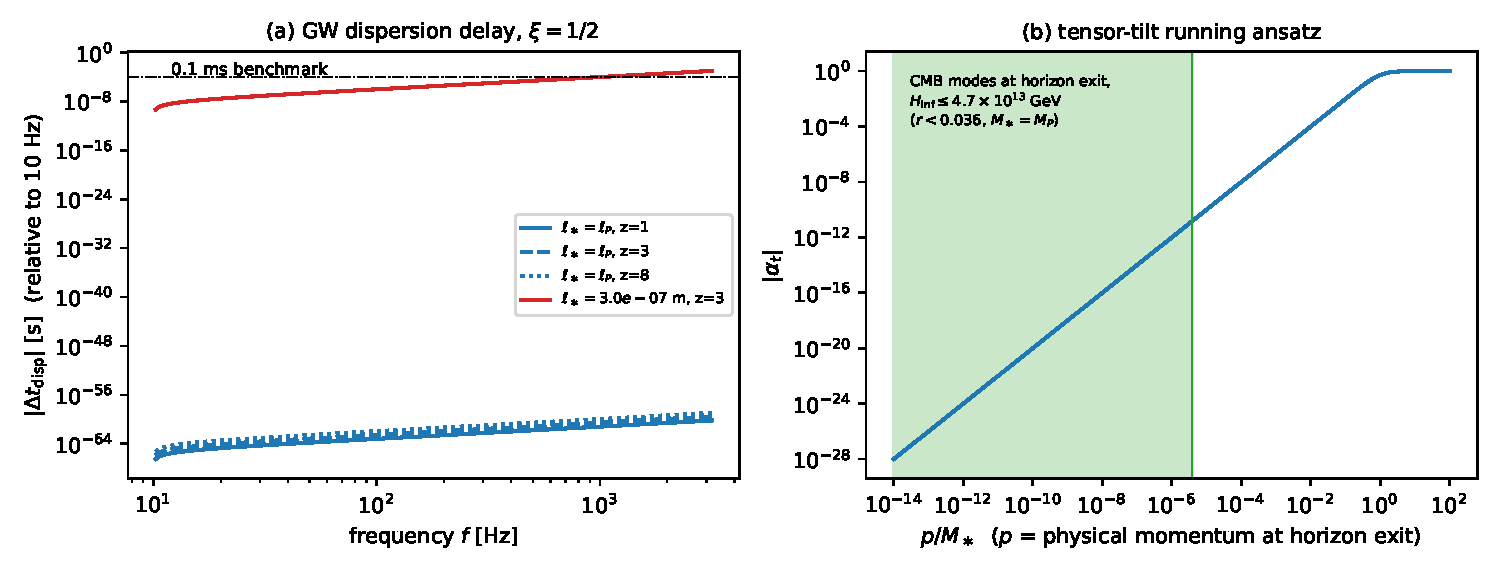
\includegraphics[width=\textwidth]{fig_observability_estimates.pdf}
\caption{\textbf{Order-of-magnitude assessment.} (a) Arrival-time delay $|\Delta t_{\mathrm{disp}}|$ relative to $10$\,Hz, Eq.~\eqref{eq:delta_t} with $\xi = 1/2$. Blue: $\ell_\ast = \ell_P$ at $z = 1, 3, 8$. Red: the value $\ell_\ast \approx 3.0 \times 10^{-7}$\,m that would be required to reach a $0.1$\,ms delay at $1$\,kHz for $z = 3$. Dash-dotted: $0.1$\,ms timing benchmark. (b) The tilt-running ansatz \eqref{eq:tensor_running} as a function of $p/M_\ast$, with $p$ the physical momentum of the mode at horizon exit. The shaded region, $p = H_{\mathrm{inf}} \le 4.7 \times 10^{13}$\,GeV, contains the CMB modes for $M_\ast = M_P$ and $r < 0.036$. Figure reproduced from \cite{silvafilho2026treatise}, Chapter~13.}
\label{fig:experimental}
\end{figure}

\begin{enumerate}[label=(\roman*),leftmargin=1.8em]
    \item \textbf{Graviton dispersion delay (ET, CE, LISA).} The running of $d_s$ does not by itself fix a dispersion relation for gravitational waves. As a phenomenological ansatz we take $\omega^2 = c^2 k^2 (1 + \xi \ell_\ast^2 k^2)$. The diffusion model of Proposition~\ref{thm:spectral_dimension_flow} suggests $\ell_\ast = \ell_P$ but does not fix $\xi$: its isotropic Lorentzian continuation has a non-dispersive massless branch ($\xi = 0$) and a ghost (Remark~\ref{rem:ds_scope}), and the anisotropic operator that would give $\xi = 1$ has $d_s \to 5/2$. We treat $\xi$ as a free parameter of order unity and display $\xi = 1/2$. The group velocity is $v_g \approx c(1 + \frac{3}{2}\xi \ell_\ast^2 k^2)$, and a graviton observed at frequency $f$ had physical wavenumber $2\pi f(1+z')/c$ at redshift $z'$, so two frequencies $f_1 < f_2$ emitted together at redshift $z$ arrive separated by \cite{jacob2008lorentz, mirshekari2012constraining}
    \begin{equation}
        \label{eq:delta_t}
        |\Delta t_{\mathrm{disp}}| = \frac{6\pi^2 \xi \ell_\ast^2}{c^3}\, D_2(z) \left(f_2^2 - f_1^2\right), \qquad D_2(z) = \frac{c}{H_0} \int_0^z \frac{(1+z')^2 \dif z'}{\sqrt{\Omega_m(1+z')^3 + \Omega_\Lambda}}.
    \end{equation}
    For $\ell_\ast = \ell_P$, $f_1 = 10$\,Hz, $f_2 = 1$\,kHz, $H_0 = 70$\,km\,s$^{-1}$\,Mpc$^{-1}$ and $\Omega_m = 0.3$ this gives $|\Delta t_{\mathrm{disp}}| \approx 6 \times 10^{-62}$, $3 \times 10^{-61}$ and $1.2 \times 10^{-60}$\,s at $z = 1, 3, 8$. Taking an optimistic timing benchmark of $10^{-4}$\,s for third-generation detectors (Einstein Telescope, Cosmic Explorer; actual dispersion tests fit the waveform phase), the signal is $56$--$57$ orders of magnitude below reach; LISA, at millihertz frequencies, is less sensitive to an $f^2$ effect. A $10^{-4}$\,s delay at $z = 3$ would require $\ell_\ast \approx 3.0 \times 10^{-7}$\,m, an energy scale $\hbar c/\ell_\ast \approx 0.7$\,eV. Nothing in the framework points to such a scale, and it would have to be confronted with existing constraints on gravitational-wave propagation, among them $|v_g - c|/c \lesssim 10^{-15}$ from GW170817 \cite{abbott2017gravitational}.

    \item \textbf{Tensor-tilt running (LiteBIRD, CMB-S4).} If one \emph{postulates} that the running of the tensor tilt tracks a two-point Pad\'e form of the spectral dimension, $d_s(p) = 2 + 2/(1 + (p/M_\ast)^2)$,
    \begin{equation}
        \label{eq:tensor_running}
        \alpha_t = \frac{1}{2}\left(d_s(p) - 4\right) = -\frac{(p/M_\ast)^2}{1 + (p/M_\ast)^2},
    \end{equation}
    the momentum $p$ must be physical. A local effect with scale $M_\ast$ acts on a tensor mode when it is generated, at horizon exit, where $p = k/a = H_{\mathrm{inf}}$; the comoving wavenumber measured today is not an invariant scale. The bound $r < 0.036$ \cite{bicepkeck2021constraints} and $A_s \approx 2.1 \times 10^{-9}$ \cite{planck2018parameters} give, through $2H_{\mathrm{inf}}^2/(\pi^2 M_{\mathrm{red}}^2) = rA_s$ with $M_{\mathrm{red}} = M_P/\sqrt{8\pi}$, the bound $H_{\mathrm{inf}} \le 4.7 \times 10^{13}$\,GeV. For $M_\ast = M_P$, $|\alpha_t| \approx (H_{\mathrm{inf}}/M_P)^2 \le 1.5 \times 10^{-11}$ ($3.7 \times 10^{-10}$ for $M_\ast = M_{\mathrm{red}}$), nearly the same for all CMB multipoles. LiteBIRD \cite{litebird2023probing} and CMB-S4 target the tensor amplitude at the level $r \sim 10^{-3}$; the ansatz predicts no observable modification of $C_\ell^{BB}$.

    \item \textbf{Quantum simulators.} Programmable Rydberg arrays \cite{ebadi2021quantum} and superconducting circuits can measure quantum Fisher metrics and out-of-time-order correlators, whose Lyapunov exponent obeys the Maldacena--Shenker--Stanford bound \cite{maldacena2016bound}. Such experiments probe the many-body systems realized; they would test the framework only if a concrete model were identified in which it makes a quantitative prediction. We do not have such a model.

    \item \textbf{Atom interferometry.} For $^{87}$Sr atoms in long-baseline instruments (MAGIS-100, AION) \cite{abe2021matter, badurina2020aion}, $\ell_P/\lambda_{\mathrm{dB}} = m v\, \ell_P/(2\pi\hbar) \approx 3.5 \times 10^{-27}\,(v/1\,\mathrm{m\,s^{-1}})$, which stays below $2 \times 10^{-25}$ for launch velocities $v \lesssim 45$\,m\,s$^{-1}$. No prediction of the framework is attached to this ratio, and no test is proposed.
\end{enumerate}

In summary, with the scale set by $\ell_P$ the observational ans\"atze give effects suppressed by factors of order $(\ell_P k)^2$ for gravitational waves and $(H_{\mathrm{inf}}/M_P)^2$ for the tensor tilt, far below current or planned experimental reach. In its present form the framework makes no observable prediction; obtaining one would require an independent mechanism that enhances Planck-suppressed effects, or a lower scale $\ell_\ast$ justified from first principles.

% =========================================================================
\section{Conclusion and Outlook}
\label{sec:conclusion}
% =========================================================================

We have separated what the Simplicial Quantum Gravity framework on $\Delta_4 \times \Delta_2$ establishes from what it suggests.
\begin{enumerate}
    \item \textbf{Established:} a closed-form spectral dimension $d_s: 4 \to 2$ for the assumed two-scale symbol $k^2 + \ell_P^2 k^4$ (Proposition~\ref{thm:spectral_dimension_flow}); sharp pointwise bounds on $K_{ij}K^{ij}$, $\sigma_{ij}\sigma^{ij}$ and ${}^{(3)}R$ on slices of bounded extrinsic curvature (Theorem~\ref{thm:minimax_shear}) and the resulting Hubble-rate and density bound in FLRW (Proposition~\ref{thm:planck_bounce}); the Clifford structure of Dirac--K\"ahler fields (Proposition~\ref{thm:nielsen_ninomiya_evasion}); Caffarelli's optimal regularity in the obstacle model (Theorem~\ref{thm:caffarelli_regularity}); and an exponential-decay estimate for the graphon Ricci flow, conditional on a curvature hypothesis whose validity depends on the chosen metric.
    \item \textbf{Conjectured:} a Yang--Mills mass gap on the Gribov region under hypotheses (H1)--(H2) (Conjecture~\ref{thm:yang_mills_gap}), and the condensation of graphon Ricci flows into smooth four-dimensional geometries (Conjecture~\ref{conj:graphon_condensation}).
    \item \textbf{Not obtained:} a bounce or any modification of the Friedmann equation; the Born rule from phase-space volumes; an evasion of fermion doubling; a derivation of three generations or of the Koide relation; a cancellation of vacuum energy from $\partial \circ \partial = 0$; a simplicial realization of the double copy.
    \item \textbf{Observationally:} Planck-suppressed signatures of the kind considered here are many orders of magnitude below experimental reach (Section~\ref{sec:experimental_signatures}).
\end{enumerate}
The framework does not, at present, constitute a UV-complete theory of quantum gravity, and the problems listed in Table~\ref{tab:fundamental_problems} remain open. Deriving the two-scale symbol from a simplicial operator, posing a well-defined minimax slicing problem with boundary conditions, and proving the conjectures above are the natural programme for future work.

% =========================================================================
% REFERENCES
% =========================================================================

\begin{thebibliography}{99}

% --- Author's Zenodo Treatises ---
\bibitem{silvafilho2026treatise}
R.~M. Silva-Filho,
\emph{Geometry, Tensors, and Quantum Gravity: Foundations of Simplicial Geometry, Minimax Foliations, and Emergent Spacetime},
Zenodo Monograph Archive, version~2.3, \href{https://doi.org/10.5281/zenodo.22290043}{DOI: 10.5281/zenodo.22290043} (all versions), 2026.

\bibitem{silvafilho2026trilogy}
R.~M. Silva-Filho,
\emph{Beyond the Spectrum: Functional Realizations of Matrices and Tensors, Emerging Invariants, and Geometric Measures (Volumes I--III)},
Zenodo Monograph Archive, \href{https://doi.org/10.5281/zenodo.22441676}{DOI: 10.5281/zenodo.22441676}, 2026.

\bibitem{silvafilho2026yangmills}
R.~M. Silva-Filho,
\emph{A Geometric and Metric-Measure Framework for the Yang--Mills Mass Gap, Gribov--Zwanziger Horizon Regularization, and Confinement on Gauge Orbit Varieties},
Zenodo Research Paper, \href{https://doi.org/10.5281/zenodo.22699843}{DOI: 10.5281/zenodo.22699843}, 2026.

\bibitem{silvafilho2026lagrangian}
R.~M. Silva-Filho,
\emph{Geometric Condensation of Fundamental Interactions: From the Classical Multi-Component Lagrangian to the Simplicial Action Functional on $\Delta_4 \times \Delta_2$},
Zenodo Research Paper, \href{https://doi.org/10.5281/zenodo.22707110}{DOI: 10.5281/zenodo.22707110}, 2026.

\bibitem{silvafilho2026fermions}
R.~M. Silva-Filho,
\emph{Geometric Foundations of the Fermion Mass Hierarchy, Flavor Mixing, and Vacuum Energy Suppression in Simplicial Spacetime},
Zenodo Research Paper, \href{https://doi.org/10.5281/zenodo.22707125}{DOI: 10.5281/zenodo.22707125}, 2026.

\bibitem{silvafilho2026cobordisms}
R.~M. Silva-Filho,
\emph{A Functorial Bridge from Continuous Tensor Manifolds to 4-Dimensional Spacetime Cobordisms},
Zenodo Monograph, \href{https://doi.org/10.5281/zenodo.22441676}{DOI: 10.5281/zenodo.22441676}, ISBN: 978-65-87456-12-8, 2026.

% --- Quantum Gravity & Dynamical Triangulations ---
\bibitem{regge1961general}
T.~Regge,
\emph{General relativity without coordinates},
Nuovo Cim. \textbf{19} (1961), 558--571, \href{https://doi.org/10.1007/BF02733251}{DOI: 10.1007/BF02733251}.

\bibitem{ambjorn2001dynamically}
J.~Ambj{\o}rn, J.~Jurkiewicz, and R.~Loll,
\emph{Dynamically triangulating Lorentzian quantum gravity},
Nucl. Phys. B \textbf{610} (2001), 347--382, \href{https://doi.org/10.1016/S0550-3213(01)00297-8}{DOI: 10.1016/S0550-3213(01)00297-8}.

\bibitem{ambjorn2005spectral}
J.~Ambj{\o}rn, J.~Jurkiewicz, and R.~Loll,
\emph{The spectral dimension of the universe is scale dependent},
Phys. Rev. Lett. \textbf{95} (2005), 171301, \href{https://doi.org/10.1103/PhysRevLett.95.171301}{DOI: 10.1103/PhysRevLett.95.171301}.

\bibitem{ambjorn2012nonperturbative}
J.~Ambj{\o}rn, A.~G{\"o}rlich, J.~Jurkiewicz, and R.~Loll,
\emph{Nonperturbative quantum gravity},
Phys. Rept. \textbf{519} (2012), 127--210, \href{https://doi.org/10.1016/j.physrep.2012.03.007}{DOI: 10.1016/j.physrep.2012.03.007}.

\bibitem{horava2009spectral}
P.~Ho\v{r}ava,
\emph{Spectral dimension of the universe in quantum gravity at a Lifshitz point},
Phys. Rev. Lett. \textbf{102} (2009), 161301, \href{https://doi.org/10.1103/PhysRevLett.102.161301}{DOI: 10.1103/PhysRevLett.102.161301}.

\bibitem{sotiriou2011spectral}
T.~P. Sotiriou, M.~Visser, and S.~Weinfurtner,
\emph{Spectral dimension as a probe of the ultraviolet continuum regime of causal dynamical triangulations},
Phys. Rev. Lett. \textbf{107} (2011), 131303, \href{https://doi.org/10.1103/PhysRevLett.107.131303}{DOI: 10.1103/PhysRevLett.107.131303}.

\bibitem{carlip2017dimension}
S.~Carlip,
\emph{Dimension and dimensional reduction in quantum gravity},
Class. Quantum Grav. \textbf{34} (2017), 193001, \href{https://doi.org/10.1088/1361-6382/aa8535}{DOI: 10.1088/1361-6382/aa8535}.

\bibitem{hamber2009quantum}
H.~W. Hamber,
\emph{Quantum Gravitation: The Feynman Path Integral Approach},
Springer, Berlin, 2009, ISBN: 978-3-540-85292-6, \href{https://doi.org/10.1007/978-3-540-85293-3}{DOI: 10.1007/978-3-540-85293-3}.

\bibitem{oriti2009approaches}
D.~Oriti (ed.),
\emph{Approaches to Quantum Gravity: Toward a New Understanding of Space, Time and Matter},
Cambridge University Press, Cambridge, 2009, ISBN: 978-0-521-51452-1, \href{https://doi.org/10.1017/CBO9780511575549}{DOI: 10.1017/CBO9780511575549}.

\bibitem{freidel2005group}
L.~Freidel,
\emph{Group field theory: An overview},
Int. J. Theor. Phys. \textbf{44} (2005), 1769--1783, \href{https://doi.org/10.1007/s10773-005-8894-1}{DOI: 10.1007/s10773-005-8894-1}.

\bibitem{ashtekar2006quantum}
A.~Ashtekar, T.~Pawlowski, and P.~Singh,
\emph{Quantum nature of the big bang: Improved dynamics},
Phys. Rev. D \textbf{74} (2006), 084003, \href{https://doi.org/10.1103/PhysRevD.74.084003}{DOI: 10.1103/PhysRevD.74.084003}.

\bibitem{goroff1986ultraviolet}
M.~H. Goroff and A.~Sagnotti,
\emph{The ultraviolet behavior of Einstein gravity},
Nucl. Phys. B \textbf{266} (1986), 709--736, \href{https://doi.org/10.1016/0550-3213(86)90193-8}{DOI: 10.1016/0550-3213(86)90193-8}.

\bibitem{hawking1970singularities}
S.~W. Hawking and R.~Penrose,
\emph{The singularities of gravitational collapse and cosmology},
Proc. R. Soc. Lond. A \textbf{314} (1970), 529--548, \href{https://doi.org/10.1098/rspa.1970.0021}{DOI: 10.1098/rspa.1970.0021}.

\bibitem{arnowitt1962dynamics}
R.~Arnowitt, S.~Deser, and C.~W. Misner,
\emph{The dynamics of general relativity},
in \emph{Gravitation: An Introduction to Current Research}, L.~Witten (ed.), Wiley, New York, 1962, pp.~227--265; republished in Gen. Relativ. Gravit. \textbf{40} (2008), 1997--2027, \href{https://doi.org/10.1007/s10714-008-0661-1}{DOI: 10.1007/s10714-008-0661-1}.

\bibitem{dirac1964lectures}
P.~A.~M. Dirac,
\emph{Lectures on Quantum Mechanics},
Belfer Graduate School of Science, Yeshiva University, New York, 1964, ISBN: 978-0-486-41713-4.

\bibitem{dewitt1967quantum}
B.~S. DeWitt,
\emph{Quantum theory of gravity. I. The canonical theory},
Phys. Rev. \textbf{160} (1967), 1113--1148, \href{https://doi.org/10.1103/PhysRev.160.1113}{DOI: 10.1103/PhysRev.160.1113}.

% --- Variational Inequalities, Obstacle Problems & Geometry ---
\bibitem{caffarelli1998obstacle}
L.~A. Caffarelli,
\emph{The obstacle problem revisited},
J. Fourier Anal. Appl. \textbf{4} (1998), 383--402, \href{https://doi.org/10.1007/BF02498216}{DOI: 10.1007/BF02498216}.

\bibitem{caffarelli2005geometric}
L.~A. Caffarelli and S.~Salsa,
\emph{A Geometric Approach to Free Boundary Problems},
Graduate Studies in Mathematics, Vol.~68, American Mathematical Society, Providence, RI, 2005, ISBN: 978-0-8218-3784-9, \href{https://doi.org/10.1090/gsm/068}{DOI: 10.1090/gsm/068}.

\bibitem{kinderlehrer1980introduction}
D.~Kinderlehrer and G.~Stampacchia,
\emph{An Introduction to Variational Inequalities and Their Applications},
Academic Press, New York, 1980; reprinted by SIAM, 2000, ISBN: 978-0-89871-466-1, \href{https://doi.org/10.1137/1.9780898719451}{DOI: 10.1137/1.9780898719451}.

\bibitem{evans1998partial}
L.~C. Evans,
\emph{Partial Differential Equations},
Graduate Studies in Mathematics, Vol.~19, American Mathematical Society, Providence, RI, 1998, ISBN: 978-0-8218-0772-9, \href{https://doi.org/10.1090/gsm/019}{DOI: 10.1090/gsm/019}.

\bibitem{federer1959curvature}
H.~Federer,
\emph{Curvature measures},
Trans. Amer. Math. Soc. \textbf{93} (1959), 418--491, \href{https://doi.org/10.1090/S0002-9947-1959-0110078-1}{DOI: 10.1090/S0002-9947-1959-0110078-1}.

% --- Gauge Theory, Gribov-Zwanziger & Confinement ---
\bibitem{faddeev1967feynman}
L.~D. Faddeev and V.~N. Popov,
\emph{Feynman diagrams for the Yang-Mills field},
Phys. Lett. B \textbf{25} (1967), 29--30, \href{https://doi.org/10.1016/0370-2693(67)90067-6}{DOI: 10.1016/0370-2693(67)90067-6}.

\bibitem{gribov1978quantization}
V.~N. Gribov,
\emph{Quantization of non-Abelian gauge theories},
Nucl. Phys. B \textbf{139} (1978), 1--19, \href{https://doi.org/10.1016/0550-3213(78)90175-X}{DOI: 10.1016/0550-3213(78)90175-X}.

\bibitem{zwanziger1989local}
D.~Zwanziger,
\emph{Local and renormalizable action from the Gribov horizon},
Nucl. Phys. B \textbf{323} (1989), 513--544, \href{https://doi.org/10.1016/0550-3213(89)90122-3}{DOI: 10.1016/0550-3213(89)90122-3}.

\bibitem{vandersickel2012gribov}
N.~Vandersickel and D.~Zwanziger,
\emph{The Gribov problem and QCD dynamics},
Phys. Rept. \textbf{520} (2012), 175--251, \href{https://doi.org/10.1016/j.physrep.2012.07.003}{DOI: 10.1016/j.physrep.2012.07.003}.

\bibitem{savvidy1977infrared}
G.~K. Savvidy,
\emph{Infrared instability of the vacuum state of gauge theories and asymptotic freedom},
Phys. Lett. B \textbf{71} (1977), 133--134, \href{https://doi.org/10.1016/0370-2693(77)90759-6}{DOI: 10.1016/0370-2693(77)90759-6}.

\bibitem{thooft1978phase}
G.~'t~Hooft,
\emph{On the phase transition towards permanent quark confinement},
Nucl. Phys. B \textbf{138} (1978), 1--25, \href{https://doi.org/10.1016/0550-3213(78)90153-0}{DOI: 10.1016/0550-3213(78)90153-0}.

\bibitem{wilson1974confinement}
K.~G. Wilson,
\emph{Confinement of quarks},
Phys. Rev. D \textbf{10} (1974), 2445--2459, \href{https://doi.org/10.1103/PhysRevD.10.2445}{DOI: 10.1103/PhysRevD.10.2445}.

\bibitem{polyakov1975compact}
A.~M. Polyakov,
\emph{Compact gauge fields and the infrared catastrophe},
Phys. Lett. B \textbf{59} (1975), 82--84, \href{https://doi.org/10.1016/0370-2693(75)90162-8}{DOI: 10.1016/0370-2693(75)90162-8}.

\bibitem{jaffe2006quantum}
A.~Jaffe and E.~Witten,
\emph{Quantum Yang--Mills Theory},
in \emph{The Millennium Prize Problems}, J.~Carlson, A.~Jaffe, and A.~Wiles (eds.), Clay Mathematics Institute / American Mathematical Society, Cambridge, MA, 2006, pp.~129--152, ISBN: 978-0-8218-3679-8.

% --- Differential Forms, Clifford Algebra & Fermions ---
\bibitem{kahler1962innere}
E.~K{\"a}hler,
\emph{Der innere Differentialkalk{\"u}l},
Rendiconti di Matematica e delle sue Applicazioni \textbf{21} (1962), 425--523.

\bibitem{becher1982dirac}
P.~Becher and H.~Joos,
\emph{The Dirac--K{\"a}hler equation and fermions on the lattice},
Z. Phys. C \textbf{15} (1982), 343--365, \href{https://doi.org/10.1007/BF01614426}{DOI: 10.1007/BF01614426}.

\bibitem{rabin1982homology}
J.~M. Rabin,
\emph{Homology theory of lattice fermion doubling},
Nucl. Phys. B \textbf{201} (1982), 315--332, \href{https://doi.org/10.1016/0550-3213(82)90434-5}{DOI: 10.1016/0550-3213(82)90434-5}.

\bibitem{banks1982geometric}
T.~Banks, Y.~Dothan, and D.~Horn,
\emph{Geometric fermions},
Phys. Lett. B \textbf{117} (1982), 413--417, \href{https://doi.org/10.1016/0370-2693(82)90571-8}{DOI: 10.1016/0370-2693(82)90571-8}.

\bibitem{nielsen1981absence}
H.~B. Nielsen and M.~Ninomiya,
\emph{Absence of neutrinos on a lattice: (I). Proof by homotopy theory},
Nucl. Phys. B \textbf{185} (1981), 20--40, \href{https://doi.org/10.1016/0550-3213(81)90361-8}{DOI: 10.1016/0550-3213(81)90361-8}.

% --- Flavor Physics & Koide Relation ---
\bibitem{koide1982fermion}
Y.~Koide,
\emph{Fermion-boson two-body model of quarks and leptons and Cabibbo mixing},
Lett. Nuovo Cim. \textbf{34} (1982), 201--205, \href{https://doi.org/10.1007/BF02817096}{DOI: 10.1007/BF02817096}.

\bibitem{koide1983fermion}
Y.~Koide,
\emph{New view of quark and lepton mass hierarchy},
Phys. Rev. D \textbf{28} (1983), 252--254, \href{https://doi.org/10.1103/PhysRevD.28.252}{DOI: 10.1103/PhysRevD.28.252}.

\bibitem{foot1994note}
R.~Foot,
\emph{A note on Koide's lepton mass relation},
Preprint (1994), \href{https://arxiv.org/abs/hep-ph/9402242}{arXiv:hep-ph/9402242}, \href{https://doi.org/10.48550/arXiv.hep-ph/9402242}{DOI: 10.48550/arXiv.hep-ph/9402242}.

\bibitem{harari1978charge}
H.~Harari, H.~Haut, and J.~Weyers,
\emph{Quark masses and Cabibbo angles},
Phys. Lett. B \textbf{78} (1978), 459--461, \href{https://doi.org/10.1016/0370-2693(78)90485-9}{DOI: 10.1016/0370-2693(78)90485-9}.

% --- Holography, Scattering Amplitudes & Entanglement ---
\bibitem{bern2008new}
Z.~Bern, J.~J.~M. Carrasco, and H.~Johansson,
\emph{New relations for gauge-theory amplitudes},
Phys. Rev. D \textbf{78} (2008), 085011, \href{https://doi.org/10.1103/PhysRevD.78.085011}{DOI: 10.1103/PhysRevD.78.085011}.

\bibitem{ryu2006holographic}
S.~Ryu and T.~Takayanagi,
\emph{Holographic derivation of entanglement entropy from AdS/CFT},
Phys. Rev. Lett. \textbf{96} (2006), 181602, \href{https://doi.org/10.1103/PhysRevLett.96.181602}{DOI: 10.1103/PhysRevLett.96.181602}.

\bibitem{hubeny2007covariant}
V.~E. Hubeny, M.~Rangamani, and T.~Takayanagi,
\emph{A covariant holographic entanglement entropy proposal},
J. High Energ. Phys. \textbf{2007} (2007), 062, \href{https://doi.org/10.1088/1126-6708/2007/07/062}{DOI: 10.1088/1126-6708/2007/07/062}.

\bibitem{faulkner2014gravitation}
T.~Faulkner, M.~Guica, T.~Hartman, R.~C. Myers, and M.~Van~Raamsdonk,
\emph{Gravitation from entanglement in holographic CFTs},
J. High Energ. Phys. \textbf{2014} (2014), 51, \href{https://doi.org/10.1007/JHEP03(2014)051}{DOI: 10.1007/JHEP03(2014)051}.

\bibitem{vanraamsdonk2010building}
M.~Van~Raamsdonk,
\emph{Building up spacetime with quantum entanglement},
Gen. Relativ. Gravit. \textbf{42} (2010), 2323--2329, \href{https://doi.org/10.1007/s10714-010-1034-0}{DOI: 10.1007/s10714-010-1034-0}.

\bibitem{maldacena2016bound}
J.~Maldacena, S.~H. Shenker, and D.~Stanford,
\emph{A bound on chaos},
J. High Energ. Phys. \textbf{2016} (2016), 106, \href{https://doi.org/10.1007/JHEP08(2016)106}{DOI: 10.1007/JHEP08(2016)106}.

\bibitem{verstraete2010renormalization}
F.~Verstraete and J.~I. Cirac,
\emph{Continuous matrix product states for quantum fields},
Phys. Rev. Lett. \textbf{104} (2010), 190405, \href{https://doi.org/10.1103/PhysRevLett.104.190405}{DOI: 10.1103/PhysRevLett.104.190405}.

\bibitem{swingle2012entanglement}
B.~Swingle,
\emph{Entanglement renormalization and holography},
Phys. Rev. D \textbf{86} (2012), 065007, \href{https://doi.org/10.1103/PhysRevD.86.065007}{DOI: 10.1103/PhysRevD.86.065007}.

% --- Formal Verification & Foundations ---
\bibitem{avigad2018mechanization}
J.~Avigad,
\emph{The mechanization of mathematics},
Notices Amer. Math. Soc. \textbf{65} (2018), 671--678, \href{https://doi.org/10.1090/noti1688}{DOI: 10.1090/noti1688}.

\bibitem{hales2017formal}
T.~Hales et~al.,
\emph{A formal proof of the Kepler conjecture},
Forum of Mathematics, Pi \textbf{5} (2017), e2, \href{https://doi.org/10.1017/fmp.2017.1}{DOI: 10.1017/fmp.2017.1}.

\bibitem{gonthier2008formal}
G.~Gonthier,
\emph{Formal proof---the four-color theorem},
Notices Amer. Math. Soc. \textbf{55} (2008), 1382--1393.

% --- Observational References & Quantum Simulation ---
\bibitem{abbott2017gravitational}
B.~P. Abbott et~al. (LIGO Scientific and Virgo Collaborations),
\emph{Gravitational waves and gamma-rays from a binary neutron star merger: GW170817 and GRB 170817A},
Astrophys. J. Lett. \textbf{848} (2017), L13, \href{https://doi.org/10.3847/2041-8213/aa920c}{DOI: 10.3847/2041-8213/aa920c}.

\bibitem{jacob2008lorentz}
U.~Jacob and T.~Piran,
\emph{Lorentz-violation-induced arrival delays of cosmological particles},
J. Cosmol. Astropart. Phys. \textbf{2008} (2008), 031, \href{https://doi.org/10.1088/1475-7516/2008/01/031}{DOI: 10.1088/1475-7516/2008/01/031}.

\bibitem{mirshekari2012constraining}
S.~Mirshekari, N.~Yunes, and C.~M. Will,
\emph{Constraining Lorentz-violating, modified dispersion relations with gravitational waves},
Phys. Rev. D \textbf{85} (2012), 024041, \href{https://doi.org/10.1103/PhysRevD.85.024041}{DOI: 10.1103/PhysRevD.85.024041}.

\bibitem{bicepkeck2021constraints}
P.~A.~R. Ade et~al. (BICEP/Keck Collaboration),
\emph{Improved constraints on primordial gravitational waves using Planck, WMAP, and BICEP/Keck observations through the 2018 observing season},
Phys. Rev. Lett. \textbf{127} (2021), 151301, \href{https://doi.org/10.1103/PhysRevLett.127.151301}{DOI: 10.1103/PhysRevLett.127.151301}.

\bibitem{planck2018parameters}
N.~Aghanim et~al. (Planck Collaboration),
\emph{Planck 2018 results. VI. Cosmological parameters},
Astron. Astrophys. \textbf{641} (2020), A6, \href{https://doi.org/10.1051/0004-6361/201833910}{DOI: 10.1051/0004-6361/201833910}.

\bibitem{litebird2023probing}
E.~Allys et~al. (LiteBIRD Collaboration),
\emph{Probing cosmic inflation with the LiteBIRD cosmic microwave background polarization satellite},
Prog. Theor. Exp. Phys. \textbf{2023} (2023), 042F01, \href{https://doi.org/10.1093/ptep/ptac150}{DOI: 10.1093/ptep/ptac150}.

\bibitem{ebadi2021quantum}
S.~Ebadi et~al.,
\emph{Quantum phases of matter on a 256-atom programmable quantum simulator},
Nature \textbf{595} (2021), 227--232, \href{https://doi.org/10.1038/s41586-021-03582-4}{DOI: 10.1038/s41586-021-03582-4}.

\bibitem{abe2021matter}
M.~Abe et~al.,
\emph{Matter-wave atomic gradiometer interferometric sensor (MAGIS-100)},
Quantum Sci. Technol. \textbf{6} (2021), 044003, \href{https://doi.org/10.1088/2058-9565/abf719}{DOI: 10.1088/2058-9565/abf719}.

\bibitem{badurina2020aion}
L.~Badurina et~al.,
\emph{AION: An Atom Interferometer Observatory and Network},
J. Cosmol. Astropart. Phys. \textbf{2020} (2020), 011, \href{https://doi.org/10.1088/1475-7516/2020/05/011}{DOI: 10.1088/1475-7516/2020/05/011}.

\end{thebibliography}

\end{document}
